
\begin{dang}{Phương trình đẳng cấp bậc $n$ đối với $\sin x$ và $\cos x$ }
		Để giải phương trình lượng giác dạng $a\sin^2x+b\sin x\cos x+c\cos^2x=d$ ta cần nhớ:
		\begin{itemize}
		\item Trường hợp 1. Xét $\cos x =0$, khi đó $\sin x = \pm 1$. Ta thay trực tiếp vào phương trình
		\begin{itemize}
		\item Nếu thỏa mãn, suy ra $x=\dfrac{\pi}{2}+k \pi$ là nghiệm và xét tiếp trường hợp 2.
		\item Nếu không thỏa mãn, ta bỏ qua và xét tiếp trường hợp 2.
		\end{itemize}
		\item  Trường hợp 2. Xét $\cos x \ne 0$, chia 2 vế phương trình cho $\cos^2 x$ ta đưa phương trình đang xét về dạng phương trình bậc hai theo $\tan x$.
		\item  Tổng hợp nghiệm ở 2 trường hợp.
	
		\begin{note}
			Chú ý khi giải phương trình trên chúng ta có thể áp dụng các công thức sau:
		\end{note}
			\begin{listEX}[3]
				\item [\ding{172}] $\dfrac{\sin x}{\cos x}=\tan x$.
				\item [\ding{173}] $ \sin 2x = 2 \sin x \cos x$
				\item [\ding{174}] $\dfrac{1}{\cos^2 x}=\tan ^2 x+1$
			\end{listEX}
			\end{itemize}
\end{dang}
\subsubsection{Ví dụ}
\begin{vd}%[TH]%[DCHT Toán 11 - KNTT -Tên Nguyễn Thanh Sang] %[1K1B4-8]
Giải phương trình $\sin ^2 x+2\cos^2 x=3\sin x \cos x.$
	\dapso{$\left\{\dfrac{\pi}{2}+k\pi;\arctan(-3)+k\pi\mid k\in \mathbb{Z}\right\}$}
	\loigiai{
		$\sin ^2 x+2\cos^2 x=3\sin x \cos x \Leftrightarrow \sin ^2 x-3\sin x \cos x+2\cos^2 x =0$.  (1)\\
		Với $x=\dfrac{\pi}{2}+k\pi,(k \in \mathbb{Z})$ thì $\cos x=0$ và $\sin^2x=1$. Phương trình (1) trở thành: $1=0$ (vô lí), vậy loại $x=\dfrac{\pi}{2}+k\pi,(k \in \mathbb{Z})$.\\
		Với $x \ne \dfrac{\pi}{2}+k\pi,(k \in \mathbb{Z})$, chia hai vế của phương trình (1) cho $\cos^2x \ne 0$ ta được:
		\allowdisplaybreaks
		\begin{eqnarray*}
			&&\dfrac{\sin^2x}{\cos^2x}-\dfrac{3\sin x \cos x}{\cos^2x}+\dfrac{2\cos^2x}{\cos^2x}=0\\
			&\Leftrightarrow& \tan^2x-3\tan x+2=0 \\
			&\Leftrightarrow &\hoac{&\tan x=1\\&\tan x=2}\\
			&\Leftrightarrow& \hoac{&x=\dfrac{\pi}{4}+k\pi\\&x=\text{arctan}2+k\pi} (k\in \mathbb{Z}).
		\end{eqnarray*}
		Vậy nghiệm của phương trình đã cho là: $x=\dfrac{\pi}{4}+k\pi,x=\text{arctan}2+k\pi, (k\in \mathbb{Z})$.
	}
\end{vd}
\begin{vd}%[TH]%[DCHT Toán 11 - KNTT -Tên Nguyễn Thanh Sang] %[1K1B4-8]
	 Giải phương trình $2 \sin^2 x+3 \sqrt{3} \sin x \cos x- \cos^2 x=2.$
	\dapso{$\left\{\dfrac{\pi}{2}+k\pi;\dfrac{\pi}{3}+k\pi\mid k\in \mathbb{Z} \right\}$}
	\loigiai{
	\allowdisplaybreaks
	\begin{eqnarray*}
		&&2 \sin^2 x+3 \sqrt{3} \sin x \cos x- \cos^2 x=2\\
		&\Leftrightarrow& 2+3 \sqrt{3} \cot x- \cot^2 x=2(1+\cot^2 x)\\
		&\Leftrightarrow& 3 \cot^2 x -3 \sqrt{3} \cot x=0\\
		&\Leftrightarrow& \hoac{&\cot x=0\\& \cot x= \sqrt{3}}\\
		&\Leftrightarrow& \hoac{&x=\dfrac{\pi}{2}+k\pi\\&x=\dfrac{\pi}{6}+k\pi}(k\in \mathbb{Z}).
	\end{eqnarray*}}
\end{vd}
\begin{vd}%[TH]%[DCHT Toán 11 - KNTT -Tên Nguyễn Thanh Sang] %[1K1B4-8]
	$\sin^2 x-3\sin x\cos x=-1.$
	\dapso{$\left\{\dfrac{\pi}{4}+k\pi;\arctan\dfrac{1}{2}+k\pi , k\in \mathbb{Z}\right\}$}
	\loigiai{
		$\sin^2 x-3\sin x\cos x=-1$ (1)\\
		Với $x=\dfrac{\pi}{2}+k\pi,(k \in \mathbb{Z})$ thì $\cos x=0$ và $\sin^2x=1$. Phương trình (1) trở thành: $1=-1$ (vô lí), vậy loại $x=\dfrac{\pi}{2}+k\pi, (k \in \mathbb{Z})$.\\
		Với $x \ne \dfrac{\pi}{2}+k\pi, (k \in \mathbb{Z})$, chia hai vế của phương trình (1) cho $\cos^2 x \ne 0$ ta được:\\
		\allowdisplaybreaks
		\begin{eqnarray*}
			&&\dfrac{\sin^2x}{\cos^2x}-\dfrac{3\sin x \cos x}{\cos^2x}=-\dfrac{1}{\cos^2x}\\
			&\Leftrightarrow& \tan^2x-3\tan x=-(1+\tan^2x) \\
			&\Leftrightarrow& 2\tan^2x-3\tan x+1=0\\
			&\Leftrightarrow& \hoac{&\tan x=1\\&\tan x=\dfrac{1}{2}}\\
			&\Leftrightarrow& \hoac{& x=\dfrac{\pi}{4}+k\pi\\& x=\arctan\dfrac{1}{2}+k\pi.}, (k\in \mathbb{Z}).
		\end{eqnarray*}
		Vậy nghiệm của phương trình đã cho là: $x=\dfrac{\pi}{4}+k\pi;x=\arctan \dfrac{1}{2}+k\pi, (k\in \mathbb{Z})$.
	}
	\end{vd}
\begin{vd}%[TH]%[DCHT Toán 11 - KNTT -Tên Nguyễn Thanh Sang] %[1K1B4-8]
	 Giải phương trình $2\sin^2 x-\sin x\cos x-\cos^2 x=2$ (1)\\
	 	\dapso{$x=\dfrac{\pi}{2}+k\pi;x=\arctan(-3)+k\pi, (k\in \mathbb{Z})$}
	 	\loigiai{
		Với $x=\dfrac{\pi}{2}+k\pi(k \in \mathbb{Z})$ thì $\cos x=0$ và $\sin^2x=1$. Phương trình (1) luôn đúng, vậy nhận $x=\dfrac{\pi}{2}+k\pi, (k \in \mathbb{Z})$ là nghiệm của phương trình.\\
		Với $x \ne \dfrac{\pi}{2}+k\pi, (k \in \mathbb{Z})$, chia hai vế của phương trình (1) cho $\cos^2 x \ne 0$ ta được:\\
		\allowdisplaybreaks
		\begin{eqnarray*}
			&&\dfrac{2\sin^2x}{\cos^2x}-\dfrac{\sin x \cos x}{\cos^2x}-\dfrac{\cos^2x}{\cos^2x}=\dfrac{2}{\cos^2x}\\ &\Leftrightarrow& 2\tan^2x-\tan x-1=2(1+\tan^2x) \\
			&\Leftrightarrow& \tan x=-3\\
			&\Leftrightarrow& x=\arctan(-3)+k\pi, (k\in \mathbb{Z}).
		\end{eqnarray*}
		Vậy nghiệm của phương trình đã cho là: $x=\dfrac{\pi}{2}+k\pi;x=\arctan(-3)+k\pi, (k\in \mathbb{Z})$.}
\end{vd}
\begin{vd}%[VDT]%[DCHT Toán 11 - KNTT -Tên Nguyễn Thanh Sang] %[1K1K4-8]
	Giải phương trình $\sin^3 x-\sqrt{3}\cos^3 x=\sin x\cos^2 x-\sqrt{3}\sin^2 x\cos x$ 
	\dapso{$\left\{\pm\dfrac{\pi}{4}+k\pi;-\dfrac{\pi}{3}+k\pi \mid k\in \mathbb{Z}\right\}$}
	\loigiai{
	Với $x=\dfrac{\pi}{2}+k\pi, (k \in \mathbb{Z})$ thì $\cos x=0$ và $\sin^2 x=1$. Phương trình đã cho không thoả mãn, vậy loại $x=\dfrac{\pi}{2}+k\pi, (k \in \mathbb{Z})$.\\
	Với $x \ne \dfrac{\pi}{2}+k\pi, (k \in \mathbb{Z})$, chia hai vế của phương trình đã cho cho $\cos^3 x \ne 0$ ta được:\\
	\allowdisplaybreaks
	\begin{eqnarray*}
		&&\dfrac{\sin^3x}{\cos^3x}-\dfrac{\sqrt{3}\cos^3 x}{\cos^3x}=\dfrac{\sin x\cos^2x}{\cos^3x}-\dfrac{\sqrt{3}\sin^2 x\cos x}{\cos^3x}\\
		&\Leftrightarrow& \tan^3x-\sqrt{3}=\tan x-\sqrt{3}\tan^2x \\
		&\Leftrightarrow& \tan^3x+\sqrt{3}\tan^2x-\tan x-\sqrt{3}=0\\
		&\Leftrightarrow& \hoac{&\tan x=1\\&\tan x=-1\\&\tan x=-\sqrt{3}}\\
		&\Leftrightarrow &\hoac{& x=\dfrac{\pi}{4}+k\pi\\& x=-\dfrac{\pi}{4}+k\pi\\&x=-\dfrac{\pi}{3}+k\pi.}, (k\in \mathbb{Z})
	\end{eqnarray*}
	Vậy nghiệm của phương trình đã cho là: $x=\pm\dfrac{\pi}{4}+k\pi,x=-\dfrac{\pi}{3}+k\pi, (k\in \mathbb{Z})$.}
\end{vd}
\begin{vd}%[VDT]%[DCHT Toán 11 - KNTT -Tên Nguyễn Thanh Sang] %[1K1K4-8]
Giải phương trình $\cos^3 x + \sin x -3\sin^2 x\cos x= 0.$\\
	\dapso{$\left\{\dfrac{\pi}{4} +k\pi,\arctan\left( 1+\sqrt{2}\right),\arctan\left( 1-\sqrt{2}\right) \mid k\in \mathbb{Z}\right\}$}
	\loigiai{
		Với $x=\dfrac{\pi}{2}+k\pi, (k \in \mathbb{Z})$ thì $\cos x=0$ và $\sin^2 x=1$.
		Suy ra loại $ x =\dfrac{\pi}{2} +k\pi, k \in \mathbb{Z}.$\\
		Với $ x \neq\dfrac{\pi}{2} +k\pi,$ chia $2$ vế của phương trình đã cho $\cos^3x \neq 0$ ta được:
		\allowdisplaybreaks
		\begin{eqnarray*}
			&& 1+\tan x(1+\tan^2 x)-3\tan^2 x=0\\
			&\Leftrightarrow& \tan^3 x-3\tan^2 x+\tan x+1=0	\\
			&\Leftrightarrow& \hoac{&\tan x=1\\&\tan x=1+\sqrt{2}\\&\tan x=1-\sqrt{2}.}
		\end{eqnarray*}
		\begin{enumerate}[$\bullet$]
			\item $\tan x=1\Leftrightarrow x =\dfrac{\pi}{4} +k\pi, k \in \mathbb{Z}.$
			\item $\tan x=1+\sqrt{2}\Leftrightarrow x =\arctan\left( 1+\sqrt{2}\right)+k\pi, k \in \mathbb{Z}.$
			\item $\tan x=1-\sqrt{2}\Leftrightarrow x =\arctan\left( 1-\sqrt{2}\right)+k\pi, k \in \mathbb{Z}.$
		\end{enumerate}
		Vậy tập nghiệm của phương trình đã cho là: $S =\left\{ \dfrac{\pi}{4} +k\pi,\arctan\left( 1+\sqrt{2}\right),\arctan\left( 1-\sqrt{2}\right), k \in \mathbb{Z} \right\}.$
	}
\end{vd}
\subsubsection{Bài tập tự luận}
\begin{bt}%[TH]%[DCHT Toán 11 - KNTT -Tên Nguyễn Thanh Sang] %[1K1B4-8]
Giải phương trình 	$\sin^2 x-3\sin x\cos x=-1.$
\dapso{$x=\dfrac{\pi}{4}+k\pi,x=\text{arctan}\dfrac{1}{2}+k\pi, (k\in \mathbb{Z}).$}
\loigiai{
	$\sin^2 x-3\sin x\cos x=-1$ (1)\\
	Với $x=\dfrac{\pi}{2}+k\pi, (k \in \mathbb{Z})$ thì $\cos x=0$ và $\sin^2x=1$. Phương trình (1) trở thành: $1=-1$ (vô lí), vậy loại $x=\dfrac{\pi}{2}+k\pi, (k \in \mathbb{Z})$.\\
	Với $x \ne \dfrac{\pi}{2}+k\pi, (k \in \mathbb{Z})$, chia hai vế của phương trình (1) cho $\cos^2 x \ne 0$ ta được:\\
	\allowdisplaybreaks
	$\begin{aligned}[t]
		\dfrac{\sin^2x}{\cos^2x}-\dfrac{3\sin x \cos x}{\cos^2x}=\dfrac{-1}{\cos^2x} &\Leftrightarrow \tan^2x-3\tan x=-(1+\tan^2x) \\
		&\Leftrightarrow 2\tan^2x-3\tan x+1=0\\
		&\Leftrightarrow \hoac{&\tan x=1\\&\tan x=\dfrac{1}{2}}\\
		&\Leftrightarrow \hoac{& x=\dfrac{\pi}{4}+k\pi\\& x=\text{arctan}\dfrac{1}{2}+k\pi}, (k\in \mathbb{Z}).
	\end{aligned}$\\
	Vậy nghiệm của phương trình đã cho là: $x=\dfrac{\pi}{4}+k\pi,x=\text{arctan}\dfrac{1}{2}+k\pi, (k\in \mathbb{Z}).$
}
\end{bt}
\begin{bt}%[TH]%[DCHT Toán 11 - KNTT -Tên Nguyễn Thanh Sang] %[1K1B4-8]
Giải phương trình $\sin^2 x-4\sin x\cos x+3\cos^2 x=0$.
\dapso{$x=\dfrac{\pi}{4}+k\pi,x=\arctan 3+k\pi, (k\in \mathbb{Z}).$}
	\loigiai{
	Xét $\cos x=0 \Rightarrow \sin^2 x=1$, không thỏa mãn phương trình.\\
	Xét $\cos x\ne 0$. Chia hai vế cho $\cos^2x$, ta được
	$$\tan^2 x-4\tan x+3=0 \Leftrightarrow \hoac{&\tan x=1\\ &\tan x=3} \Leftrightarrow \hoac{&x=\dfrac{\pi}{4}+k\pi\\ &x=\arctan 3 +k\pi} (k\in \mathbb{Z}).$$
	Vậy tập nghiệm là $S=\biggl\{\dfrac{\pi}{4}+k\pi;\ \arctan 3+k\pi\Big|\ k\in \mathbb{Z}\biggr\}$.
		}
	\end{bt}
\begin{bt}%[TH]%[DCHT Toán 11 - KNTT -Tên Nguyễn Thanh Sang] %[1K1B4-8]
Giải phương trình $\sin^2x- \sin 2x-3 \cos^2x=0.$ 
\dapso{$x=-\dfrac{\pi}{4}+k \pi, x= \arctan 3+k \pi, (k\in \mathbb{Z}).$}
	\loigiai{
		Ta có $ \sin^2x- \sin 2x-3 \cos^2x=0 \Leftrightarrow \sin^2x-2 \sin x \cos x-3 \cos^2x=0$ (*) \\
		Do $ \cos x=0$ không thoả mãn phương trình (*) nên $ \cos x \neq 0$. \\
		Chia cả 2 vế của phương trình (*) cho $ \cos^2x$ ta được: \\
		$ \tan^2x-2 \tan x-3=0 \Leftrightarrow \left[
		\begin{aligned}
			& \tan x=-1 \\
			& \tan x=3
		\end{aligned} \right. \Leftrightarrow \left[
		\begin{aligned}& x=- \dfrac{\pi}{4}+k \pi \\& x= \arctan 3+k \pi \end{aligned} \right.~(k \in \mathbb{Z})$.
				}
\end{bt}
\begin{bt}%[TH]%[DCHT Toán 11 - KNTT -Tên Nguyễn Thanh Sang] %[1K1B4-8]
Giải phương trình $4\sqrt{3} \sin x \cos x +4 \cos^2 x=2 \sin^2 x+\dfrac{5}{2}.$
\dapso{$x=-\dfrac{\pi}{3}+k\pi, x= \arctan \dfrac{-\sqrt{3}}{9}+k\pi, (k\in \mathbb{Z}).$}
	\loigiai{
		pt $\Leftrightarrow 4\sqrt{3} \tan x+4=2 \tan^2 x+ \dfrac{5(1+ \tan^2 x)}{2}\\
		\Leftrightarrow \dfrac{9 \tan^2 x}{2}-4\sqrt{3} \tan x - \dfrac{3}{2}=0\\
		\Leftrightarrow \hoac{&\tan x=-\sqrt{3}\\& \tan x=\dfrac{\sqrt{3}}{9}}\\
		\Leftrightarrow \hoac{&\tan x=-\sqrt{3}\\& \tan x=\dfrac{\sqrt{3}}{9}} \Leftrightarrow \hoac{&x=-\dfrac{\pi}{3}+k\pi\\&x= \arctan \dfrac{-\sqrt{3}}{9}+k\pi}$}
\end{bt}
\begin{bt}%[VDT]%[DCHT Toán 11 - KNTT -Tên Nguyễn Thanh Sang] %[1K1K4-8] 
Giải phương trình $\sin^3 x-\sqrt{3}\cos^3 x=\sin x\cos^2 x-\sqrt{3}\sin^2 x\cos x.$
\dapso{$\left\{\pm\dfrac{\pi}{4}+k\pi;-\dfrac{\pi}{3}+k\pi,~ k\in \mathbb{Z}\right\}$}
	\loigiai{
		$\sin^3 x-\sqrt{3}\cos^3 x=\sin x\cos^2 x-\sqrt{3}\sin^2 x\cos x$ (1)\\
		Với $x=\dfrac{\pi}{2}+k\pi,~(k \in \mathbb{Z})$ thì $\cos x=0$ và $\sin^2x=1$. Phương trình đã cho không thoả, nên loại $x=\dfrac{\pi}{2}+k\pi,~(k \in \mathbb{Z})$.\\
		Với $x \ne \dfrac{\pi}{2}+k\pi,~(k \in \mathbb{Z})$, chia hai vế của phương trình (1) cho $\cos^3 x \ne 0$ ta được:\\
		\allowdisplaybreaks
		\begin{eqnarray*}
			&&\dfrac{\sin^3x}{\cos^3x}-\dfrac{\sqrt{3}\cos^3 x}{\cos^3x}=\dfrac{\sin x\cos^2x}{\cos^3x}-\dfrac{\sqrt{3}\sin^2 x\cos x}{\cos^3x}\\
			&\Leftrightarrow& \tan^3x-\sqrt{3}=\tan x-\sqrt{3}\tan^2x \\
			&\Leftrightarrow& \tan^3x+\sqrt{3}\tan^2x-\tan x-\sqrt{3}=0\\
			&\Leftrightarrow& \hoac{&\tan x=1\\&\tan x=-1\\&\tan x=-\sqrt{3}}\\
			&\Leftrightarrow &\hoac{& x=\dfrac{\pi}{4}+k\pi\\& x=-\dfrac{\pi}{4}+k\pi\\&x=-\dfrac{\pi}{3}+k\pi.},~(k\in \mathbb{Z})
		\end{eqnarray*}
		Vậy nghiệm của phương trình đã cho là: $x=\pm\dfrac{\pi}{4}+k\pi,x=-\dfrac{\pi}{3}+k\pi,~(k\in \mathbb{Z})$.
	}
\end{bt}
\begin{bt}%[VDT]%[DCHT Toán 11 - KNTT -Tên Nguyễn Thanh Sang]%[1K1K4-8] 
Giải phương trình $5\sin 2x\cos 2x-\cos^2 2x=0.$
\dapso{$\left\{\dfrac{\pi}{4} +k\dfrac{\pi}{2},\dfrac{1}{2}\arctan\left(\dfrac{1}{5} \right)+k\dfrac{\pi}{2} \mid k\in \mathbb{Z}\right\}$}
	\loigiai{
		Với $ x =\dfrac{\pi}{4} +k\dfrac{\pi}{2}$ thì $\cos 2x = 0$\\
		(2)$\Rightarrow 0=0$: (luôn đúng).\\
		Suy ra nhận $ x =\dfrac{\pi}{4} +k\dfrac{\pi}{2}, k \in \mathbb{Z}.$\\
		Với $ x \neq\dfrac{\pi}{4} +k\dfrac{\pi}{2},$ chia $2$ vế của (2) cho $\cos^2 2x \neq 0$ ta được:
		\allowdisplaybreaks
		\begin{eqnarray*}
			&& 5\tan 2x-1=0\\
			&\Leftrightarrow& \tan 2x=\dfrac{1}{5}	\\
			&\Leftrightarrow& 2x=\arctan\left(\dfrac{1}{5} \right)+k\pi, k \in \mathbb{Z}\\
			&\Leftrightarrow& x=\dfrac{1}{2}\arctan\left(\dfrac{1}{5} \right)+k\dfrac{\pi}{2},~ k \in \mathbb{Z}.
		\end{eqnarray*}
		Vậy tập nghiệm của phương trình đã cho là: $S =\left\{ \dfrac{\pi}{4} +k\dfrac{\pi}{2},\dfrac{1}{2}\arctan\left(\dfrac{1}{5} \right)+k\dfrac{\pi}{2}, k \in \mathbb{Z} \right\} $.
	}
\end{bt}
\begin{bt}%[TH]%[DCHT Toán 11 - KNTT -Tên Nguyễn Thanh Sang] %[1K1K4-8]
Tìm số nghiệm của phương trình $ 4\sin ^22x-3\sin 2x\cos 2x-\cos ^22x=0$ trong khoảng $ (0;\pi ).$
\dapso{Có $3$ nghiệm.} ~
	\loigiai{
	Dễ thấy $ \cos 2x=0$ không thỏa mãn phương trình. Do đó, phương trình đã cho tương đương với:\\
	$ 4{\tan }^22x-3\tan 2x-1=0$
	$\Leftrightarrow \left[
	\begin{aligned}
		&\tan 2x=1\\
		&\tan 2x=-\dfrac{1}{4}\\
	\end{aligned}\right.$
	$ \Leftrightarrow \left[
	\begin{aligned}
		&x=\dfrac{\pi }{8}+k\dfrac{\pi }{2} ~~(1)\\
		&x=\dfrac{1}{2}\arctan \left(-\dfrac{1}{4}\right)+k\dfrac{\pi }{2} ~~(2)\\
	\end{aligned}\right.$\\
	Xét $ (1)$, vì $ x\in (0;\pi )$ $ \Rightarrow 0<\dfrac{\pi }{8}+k\dfrac{\pi }{2}<\pi $ $ \Rightarrow k\in \left\{1\right\}$ (do $ k\in \mathbb{Z}$).\\
	Xét $ (2)$, vì $ x\in (0;\pi )$ $ \Rightarrow 0<\dfrac{1}{2}\arctan \left(-\dfrac{1}{4}\right)+k\dfrac{\pi }{2}<\pi $ $ \Rightarrow k\in \left\{1;2\right\}$ (do $ k\in \mathbb{Z}$).\\
	Do đó, trong khoảng $ (0;\pi )$ thì phương trình đã cho có $ 3$ nghiệm.
		}
\end{bt}
\begin{bt}%[VDC]%[DCHT Toán 11 - KNTT -Tên Nguyễn Thanh Sang] %[1K1G4-8] 
$8 \cos ^{3}\left(x+\dfrac{\pi}{3}\right)=\cos 3 x$.
\dapso{$\dfrac{\pi}{6}  + k\pi, k\pi,-\dfrac{2\pi}{3} + k\pi$}
\loigiai{
	Đặt $t=x+\dfrac{\pi}{3}$ thì $\cos 3x = \cos (3t - \pi) = -\cos 3t = 3\cos t - 4 \cot^3 t$.\\
	Khi đó phương trình trở thành:
	\begin{eqnarray*}
		8\cos^3 t = 3\cos t - 4\cos^3 t &\Leftrightarrow &3\cos t(4\cos^2 t - 1) = 0\\
		&\Leftrightarrow &\cos t(2\cos 2t + 1) = 0\\
		&\Leftrightarrow &\hoac{
			&\cos t = 0\\ &\cos 2t = -\dfrac{1}{2} = \cos\dfrac{2\pi}{3}}\\
		&\Leftrightarrow &\hoac{
			&t = \dfrac{\pi}{2} + k\pi\\ &2t = \pm\dfrac{2\pi}{3} + k2\pi
			\Leftrightarrow t = \pm\dfrac{\pi}{3} + k\pi.}
	\end{eqnarray*}
	Khi đó $x=\dfrac{\pi}{6} + k\pi$ hoặc $x=k\pi$ hoặc $x=-\dfrac{2\pi}{3} + k\pi$ với $k\in\mathbb{Z}$.\\
	Vậy tập nghiệm của phương trình là
	$S = \left\lbrace \dfrac{\pi}{6}  + k\pi, k\pi,-\dfrac{2\pi}{3} + k\pi\ \middle| \ k\in\mathbb{Z} \right\rbrace.$}
\end{bt}
\subsubsection{Bài tập trắc nghiệm}
\Opensolutionfile{ans}[ans/ans-1K1-4-Dang8]
%Cau 1
\begin{ex}%[DCHT Toán 11 - KNTT -Tên Nguyễn Thanh Sang] %[1K1Y4-8]
Phương trình $2\sin^2x-4\sin x\cos x+4\cos^2x=1$ tương đương với phương trình
\choice
{$\cos2x-2\sin2x=2$}
{$\sin2x-2\cos2x=2$}
{\True $\cos2x-2\sin2x=-2$}
{$\sin2x-2\cos2x=-2$}
\loigiai{
	\begin{align*}
		2\sin^2x-4\sin x\cos x+4\cos^2x=1&\Leftrightarrow 1-\cos2x-2\sin2x+2(1+\cos2x)=1\\
		&\Leftrightarrow\cos2x-2\sin2x=-2.
	\end{align*}
}
\end{ex}
%Cau 2
\begin{ex}%[DCHT Toán 11 - KNTT -Tên Nguyễn Thanh Sang] %[1K1Y4-8]
	Phương trình nào sau đây có tập nghiệm trùng với tập nghiệm của phương trình \\
	 $3\sin^2 x+2\sin x\cos x -5\cos^2 x=0$?
	\choice
	{$2\tan^2 x+3\tan x-5=0$}
	{$5\tan^2 x-2\tan x-3=0$}
	{$\tan x=-\dfrac{5}{3}$}
	{\True $3\tan^2 x+2\tan x-5=0$}
	\loigiai{
		\begin{itemize}
			\item Xét $\cos x =0$ suy ra $3=0$ (vô lý).
			\item Xét $\cos x \neq 0$, chia hai vế của phương trình cho $\cos^2x$, Lúc đó phương trình đã cho trở thành $3\tan^2 x+2\tan x-5=0$.
		\end{itemize}
	}
\end{ex}
%Cau 3 
\begin{ex}%[DCHT Toán 11 - KNTT -Tên Nguyễn Thanh Sang] %[1K1Y4-8]
Cho phương trình $2\sin^2x-\sin 2x-5\cos^2x-1=0$. Khi đặt $t=\tan  x,$ phương trình đã cho trở thành phương trình nào dưới đây?
\choice
{$2t^2-t-6=0$}
{$t^2-t-3=0$}
{\True $t^2-2t-6=0$}
{$t^2-t-6=0$}
\loigiai{
	\textbf{TH1:} $\cos x=0$.\\
	PT $\Leftrightarrow 2\sin^2x-2\sin x\cos x-5\cos^2x-1=0\Leftrightarrow 2\sin^2x-1=0\Leftrightarrow \sin^2x=\dfrac{1}{2}$ (vô lý).\\
	Suy ra $\cos x=0$ không phải là nghiệm của phương trình.\\
	\textbf{TH2:} $\cos x\ne 0$. Chia cả 2 vế của phương trình cho $\cos^2x$ ta được\\
	\allowdisplaybreaks{\begin{eqnarray*}
			\text{PT}	&\Leftrightarrow&  2\cdot \dfrac{\sin^2x}{\cos^2x}-\dfrac{2\sin x\cos x}{\cos^2x}-\dfrac{5\cos^2x}{\cos^2x}-\dfrac{1}{\cos^2x}=0 \\
			&\Leftrightarrow& 2\tan^2x-2\tan x-5-\left(1+\tan^2x\right)=0 \\
			&\Leftrightarrow& \tan^2x-2\tan x-6=0.
	\end{eqnarray*}}
	Với $t=\tan x$ phương trình tương đương $t^2-2t-6=0$.
}
\end{ex}
%Cau 4
\begin{ex}%[DCHT Toán 11 - KNTT -Tên Nguyễn Thanh Sang] %[1K1Y4-8]
Khi đặt $t=\tan x$ thì phương trình $\sin^2x+2\sin x\cos x-3\cos^2x=0$ trở thành phương trình nào sau đây?
\choice{\True $t^2+2t-3=0$}
{$-3t^2+2t+1=0$} 
{$t^2-2t+3=0$}
{$-3t^2-2t+1=0$}
\loigiai{
	Ta có $\cos x=0 \Leftrightarrow x=\dfrac{\pi}{2}+k\pi$ không phải là nghiệm của phương trình.\\
	Chia hai vế cho $\cos x$, phương trình đã cho tương đương $\tan^2x+2\tan x-3=0$.\\
	Đặt $t=\tan x$, phương trình đã cho trở thành $t^2+2t-3=0$.
}
\end{ex}
%Cau 5
\begin{ex}%[DCHT Toán 11 - KNTT -Tên Nguyễn Thanh Sang] %[1K1B4-8]
Giải phương trình $ 2\sin ^2x+\sqrt{3}\sin 2x=3$.
\choice
{ \True $ x=\dfrac{\pi }{3}+k\pi $}
{ $ x=\dfrac{4\pi }{3}+k\pi $}
{ $ x=\dfrac{5\pi }{3}+k\pi $}
{ $ x=\dfrac{2\pi }{3}+k\pi $}
\loigiai {
	Cách 1:\\ Xét $ \cos x=0:$ Phương trình tương đương $ 2=3$(không thỏa mãn)\\
	Xét $ \cos x\ne 0$, chia cả hai vế cho $ \cos ^2x$ ta có:\\
	$ 2{\tan }^2x+2\sqrt{3}\tan x=3({\tan }^2x+1)\Leftrightarrow {\tan }^2x-2\sqrt{3}\tan x+3=0$
	$ \Leftrightarrow \tan x=\sqrt{3}\Leftrightarrow $$ x=\dfrac{\pi }{3}+k\pi ,k\in \mathbb{Z}$\\
	Cách 2:\\ Phương trình $\Leftrightarrow -(1-2\sin ^2x)+\sqrt{3}\sin 2x=2$$ \Leftrightarrow 2\sin \left(2x-\dfrac{\pi }{6}\right)=2$$ \Leftrightarrow x=\dfrac{\pi }{3}+k\pi $}
\end{ex}
%Cau 6
\begin{ex}%[DCHT Toán 11 - KNTT -Tên Nguyễn Thanh Sang] %[1K1B4-8]
Các nghiệm của phương trình $\sin^2{x}+3 \sin{x} \cos{x}-6 \cos^2{x}=-1$ là
\choice{$\hoac{& x=-\dfrac{\pi}{4}+k\pi\\ &x=\mathrm{arctan}{\left(-\dfrac{5}{2}\right)}+k\pi}(k\in \mathbb{Z})$}
{\True $\hoac{& x=\dfrac{\pi}{4}+k\pi\\ &x=\mathrm{arctan}{\left(-\dfrac{5}{2}\right)}+k\pi}(k\in \mathbb{Z})$}
{$\hoac{& x=\dfrac{\pi}{4}+k\pi\\ &x={\left(-\dfrac{5}{2}\right)}+k\pi}(k\in \mathbb{Z})$}
{$\hoac{& x=\dfrac{\pi}{4}+k\pi\\ &x=\mathrm{arctan}{\left(\dfrac{5}{2}\right)}+k\pi}(k\in \mathbb{Z})$}
\loigiai{\allowdisplaybreaks
	\begin{align*}
		&\sin^2{x}+3 \sin{x} \cos{x}-6 \cos^2{x}=-1 \tag{3}\\
		\Leftrightarrow\ &2\sin^2{x}+3 \sin{x} \cos{x}-5 \cos^2{x}=0\\
		\Leftrightarrow\ &2\sin{x}\left( \sin{x}- \cos{x}\right)+5 \cos{x} \left(\sin{x}- \cos{x} \right)=0\\
		\Leftrightarrow\ &\left(\sin{x}- \cos{x}\right)\left(2\sin{x}+ 5\cos{x} \right)=0\\
		\Leftrightarrow\ &\hoac{&\sin{x}- \cos{x}=0\\ &2\sin{x}+5 \cos{x}=0}\\
		\Leftrightarrow\ &\hoac{&\tan{x}=1 \\&\tan{x}=-\dfrac{5}{2}}\\
		\Leftrightarrow\ &\hoac{& x=\dfrac{\pi}{4}+k\pi\\ &x=\mathrm{arctan}{\left(-\dfrac{5}{2}\right)}+k\pi}(k\in \mathbb{Z}).
\end{align*}}
\end{ex}
%Cau 7
\begin{ex}%[DCHT Toán 11 - KNTT -Tên Nguyễn Thanh Sang] %[1K1B4-8]
	Phương trình $\left(\sqrt{3}+1\right){\sin }^{2}x-2\sqrt{3}\sin x\cos x+\left(\sqrt{3}-1\right){\cos }^{2}x=0$ có các nghiệm là:
	\choice
	{$\left[
		\begin{aligned}
			&x=-\dfrac{\pi }{4}+k\pi \\
			&x=\alpha +k\pi \quad \\
		\end{aligned}\right.$(với $\tan \alpha =-2+\sqrt{3}$)}
	{\True $\left[
		\begin{aligned}
			&x=\dfrac{\pi }{4}+k\pi \\
			&x=\alpha +k\pi \\
		\end{aligned}\right.$ (với $\tan \alpha =2-\sqrt{3}$)}
	{$\left[
		\begin{aligned}
			&x=-\dfrac{\pi }{8}+k\pi \\
			&x=\alpha +k\pi \\
		\end{aligned}\right.$(với $\tan \alpha =-1+\sqrt{3}$)}
	{$\left[
		\begin{aligned}
			&x=\dfrac{\pi }{8}+k\pi \\
			&x=\alpha +k\pi \quad \\
		\end{aligned}\right.$(với $ \tan \alpha =1-\sqrt{3}$)}
	\loigiai{
		Do $\cos x=0$ không thỏa mãn phương trình, nên ta có:\\
		$\left(\sqrt{3}+1\right){\sin }^{2}x-2\sqrt{3}\sin x\cos x+\left(\sqrt{3}-1\right){\cos }^{2}x=0$\\
		$\Leftrightarrow \left(\sqrt{3}+1\right){\tan }^{2}x-2\sqrt{3}\tan x+\sqrt{3}-1=0$\\
		$\Leftrightarrow \left[
		\begin{aligned}
			&\tan x=1\\
			&\tan x=\dfrac{\sqrt{3}-1}{\sqrt{3}+1}=2-\sqrt{3}\\
		\end{aligned}\right.\Leftrightarrow \left[
		\begin{aligned}
			&x=\dfrac{\pi }{4}+k\pi \\
			&x=\alpha +k\pi \\
		\end{aligned}\right.$ (với $\tan \alpha =2-\sqrt{3}$)}
\end{ex}
%Cau 8
\begin{ex}%[DCHT Toán 11 - KNTT -Tên Nguyễn Thanh Sang] %[1K1B4-8]
Phương trình $2\sin^2x+\sin x\cos x-\cos^2x=0$ có nghiệm là
\choice
{$-\dfrac{\pi}{4}+k\pi,\arctan \left(-\dfrac{1}{2}\right)+k\pi,k \in \mathbb{Z}$}
{$\dfrac{\pi}{4}+k\pi,k \in \mathbb{Z}$}
{\True $-\dfrac{\pi}{4}+k\pi,\arctan \left(\dfrac{1}{2}\right)+k\pi,k \in \mathbb{Z}$}
{$\dfrac{\pi}{4}+k\pi,\arctan \left(\dfrac{1}{2}\right)+k\pi,k \in \mathbb{Z}$}
\loigiai{
	Ta có phương trình: $2\sin^2x+\sin x\cos x-\cos^2x=0(*)$
	\begin{itemize}
		\item Ta thấy $\cos x=0 \Rightarrow \sin x=\pm 1$ nên không thỏa phương trình $(*)$.\\
		\item Với $\cos x \ne 0$ chia hai vế phương trình $(*)$ cho $\cos^2x$ ta được\\
		$2\tan^2x+\tan x-1=0 \Leftrightarrow \hoac{&\tan x=-1 \\& \tan x=\dfrac{1}{2}}\Leftrightarrow \hoac{&x=-\dfrac{\pi}{4}+k\pi \\& x=\arctan \left(\dfrac{1}{2}\right)+k\pi },k \in \mathbb{Z}$.
\end{itemize} }
\end{ex}
%Cau 9
\begin{ex}%[DCHT Toán 11 - KNTT -Tên Nguyễn Thanh Sang] %[1K1B4-8]
Giải phương trình $ {\sin }^{2}x-\left(\sqrt{3}+1\right)\sin x\cos x+\sqrt{3}{\cos }^{2}x=0.$
\choice
{$ x=\dfrac{\pi }{3}+k2\pi \text{ }\left(k\in \mathbb{Z}\right)$}
{$ x=\dfrac{\pi }{4}+k\pi \text{ }\left(k\in \mathbb{Z}\right)$}
{$\left[
	\begin{aligned}
		&x=\dfrac{\pi }{3}+k2\pi \\
		&x=\dfrac{\pi }{4}+k2\pi \\
	\end{aligned}\right.\text{ }\left(k\in \mathbb{Z}\right)$}
{\True $\left[
	\begin{aligned}
		&x=\dfrac{\pi }{3}+k\pi \\
		&x=\dfrac{\pi }{4}+k\pi \\
	\end{aligned}\right.\text{ }\left(k\in \mathbb{Z}\right)$}
\loigiai{
	Do $\cos x=0$ không thỏa mãn phương trình, nên
	phương trình đã cho tương đương\\ $ {\tan }^{2}x-\left(\sqrt{3}+1\right)\tan x+\sqrt{3}~=0\Leftrightarrow \left[
	\begin{aligned}
		&\tan x=1\\
		&\tan x=\sqrt{3}\\
	\end{aligned}\right.$
	$ \Leftrightarrow \left[
	\begin{aligned}
		&x=\dfrac{\pi }{4}+k\pi \\
		&x=\dfrac{\pi }{3}+k\pi \\
	\end{aligned}\right.\left(k\in \mathbb{Z}\right).$}
\end{ex}
%Cau 10
\begin{ex}%[DCHT Toán 11 - KNTT -Tên Nguyễn Thanh Sang] %[1K1B4-8]
Tập nghiệm của phương trình $\sin^2 x+2\cos^2 x=\dfrac{3}{2}\sin 2x$ là
\choice{$\left\{\arctan 2+k\pi;\dfrac{\pi}{4}+k2\pi \Big| k\in\mathbb{Z}\right\}$}
{$\left\{\arctan 2+k2\pi;\dfrac{\pi}{4}+k2\pi\Big| k\in\mathbb{Z}\right\}$}
{\True $\left\{\arctan 2+k\pi;\dfrac{\pi}{4}+k\pi\Big| k\in\mathbb{Z}\right\}$}
{$\left\{\dfrac{\pi}{4}+k\pi\Big| k\in\mathbb{Z}\right\}$}
\loigiai{
	Phương trình đã cho tương đương
	$$\sin^2 x-3\sin x\cos x+2\cos^2 x=0\Leftrightarrow (\sin x-\cos x)(\sin x-2\cos x)=0.$$
	Với $\sin x=\cos x\Leftrightarrow \tan x=1\Leftrightarrow x=\dfrac{\pi}{4}+k\pi~(k\in\mathbb{Z})$.\\
	Với $\sin x=2\cos x\Leftrightarrow \tan x=2\Leftrightarrow x=\arctan 2+k\pi~(k\in\mathbb{Z})$.
}
\end{ex}
%Cau 11
\begin{ex}%[DCHT Toán 11 - KNTT -Tên Nguyễn Thanh Sang] %[1K1K4-8]
Số nghiệm của phương trình $ {\cos }^{2}x-3\sin x\cos x+2{\sin }^{2}x=0$ trên $ \left(-2\pi ;2\pi \right)$?
\choice
{$2$}
{$4$}
{$6$}
{\True$8$}
\loigiai{
	Do $\cos x=0$ không thỏa mãn phương trình, nên
	phương trình đã cho tương đương\\
	 $ 1-3\tan x+2{\tan }^{2}x=0\Leftrightarrow \left[
	\begin{aligned}
		&\tan x=1\\
		&\tan x=\dfrac{1}{2}\\
	\end{aligned}\right.\Leftrightarrow \left[
	\begin{aligned}
		&x=\dfrac{\pi }{4}+k\pi \\
		&x=\arctan \dfrac{1}{2}+k\pi \\
	\end{aligned}\right..$\\
	Vì $ x\in \left(-2\pi ;2\pi \right)\to -2\pi <\dfrac{\pi }{4}+k\pi <2\pi \to -\dfrac{9}{4}<k<\dfrac{7}{4}\xrightarrow{k\in \mathbb{Z}}k\in \left\{-2;-1;0;1\right\}$.\\
	Vì $ x\in \left(-2\pi ;2\pi \right)\to -2\pi <\arctan \dfrac{1}{2}+k\pi <2\pi $.\\
	$ \xrightarrow[\text{xấp xỉ}]{\text{CASIO}}-28,565<k<-24,565\xrightarrow{k\in \mathbb{Z}}k\in \left\{-28;-27;-26;-25\right\}$.
	Vậy có tất cả 8 nghiệm.
}
\end{ex}
%Cau 12
\begin{ex}%[DCHT Toán 11 - KNTT -Tên Nguyễn Thanh Sang]  %[1K1K4-8]
Nghiệm âm lớn nhất của phương trình $2{\sin }^{2}x+\left(1-\sqrt{3}\right)\sin x\cos x+\left(1-\sqrt{3}\right){\cos }^{2}x=1$ là:
\choice
{\True $-\dfrac{\pi }{4}$}
{$-\dfrac{2\pi }{3}$}
{$-\dfrac{\pi }{12}$}
{$-\dfrac{\pi }{6}$}
\loigiai{
	Phương trình đã cho tương đương $2{\sin }^{2}x+\left(1-\sqrt{3}\right)\sin x\cos x+\left(1-\sqrt{3}\right){\cos }^{2}x={\sin }^{2}x+{\cos }^{2}x$.\\
	$ \Leftrightarrow {\sin }^{2}x+\left(1-\sqrt{3}\right)\sin x\cos x-\sqrt{3}{\cos }^{2}x=0$.\\
	$ \Leftrightarrow {\tan }^{2}x+\left(1-\sqrt{3}\right)\tan x-\sqrt{3}=0\Leftrightarrow \left[
	\begin{aligned}
		&\tan x=-1\\
		&\tan x=\sqrt{3}\\
	\end{aligned}\right.\Leftrightarrow \left[
	\begin{aligned}
		&x=-\dfrac{\pi }{4}+k\pi \\
		&x=\dfrac{\pi }{3}+k\pi \\
	\end{aligned}\right.$.\\
	$ \xrightarrow{\text{Cho $x<0$}}\left[
	\begin{aligned}
		&-\dfrac{\pi }{4}+k\pi <0\Leftrightarrow k<\dfrac{1}{4}\xrightarrow{k\in \mathbb{Z}}{k}_{\max }=0\to x=-\dfrac{\pi }{4}\\
		&\dfrac{\pi }{3}+k\pi <0\Leftrightarrow k<-\dfrac{1}{3}\xrightarrow{k\in \mathbb{Z}}{k}_{\max }=-1\to x=-\dfrac{2\pi }{3}\\
	\end{aligned}\right..$\\
	So sánh hai nghiệm ta được $x=-\dfrac{\pi }{4}$ là nghiệm âm lớn nhất.
}
\end{ex}
%Cau 13
\begin{ex}%[DCHT Toán 11 - KNTT -Tên Nguyễn Thanh Sang]  %[1K1K4-8]
Trong khoảng $\left(0;\dfrac{\pi}{2}\right)$ phương trình ${\cos ^3}x - 3{\sin ^2}x\cos x + \sin x = 0$ có bao nhiêu nghiệm?
\choice
{\True 1}
{2}
{3}
{4}
\loigiai { Do $\cos x=0$ không là nghiệm nên phương trình tương đương\\
	$1-3\tan^2x+\tan^3x + \tan x=0$
	$\Leftrightarrow \left[
	\begin{aligned}
		&\tan x=1\\
		&\tan x=1+\sqrt{2}\\
		&\tan x=1-\sqrt{2}\\
	\end{aligned}\right.\Leftrightarrow \left[
	\begin{aligned}
		&x=\dfrac{\pi }{4}+k\pi \\
		&x=\dfrac{3\pi }{8}+k\pi \\
		&x=-\dfrac{\pi }{8}+k\pi \\
	\end{aligned}\right.$\\
	Vậy có $1$ nghiệm $x=\dfrac{\pi}{4}$ thỏa.}
\end{ex}
%Cau 14
\begin{ex}%[DCHT Toán 11 - KNTT -Tên Nguyễn Thanh Sang] %[1K1G4-8]
Tìm tất cả giá trị của tham số $m$ sao cho phương trình $\sin^4x +\cos^4x +\dfrac{1}{4} \sin 4x - (2m+1)\sin^2x \cos^2x =0$ có đúng 2 nghiệm thuộc khoảng $\left ( \dfrac{\pi}{4}; \dfrac{\pi}{2} \right  )$.
\choice
{\True $\dfrac{3}{8} < m< \dfrac{1}{2}$}
{$0 < m< 1$}
{$\dfrac{3}{4} < m< \dfrac{7}{8}$}
{$-\dfrac{1}{4} < m< \dfrac{1}{4}$}
\loigiai{
	\begin{align*}
		& \sin^4x +\cos^4x +\dfrac{1}{4} \sin 4x - (2m+1)\sin^2x \cos^2x =0 \\
		\Leftrightarrow&  1-\dfrac{1}{2} \sin^22x+ \dfrac{1}{2} \sin 2x \cos 2x -\dfrac{(2m+1)\sin^22x}{4} \\
		\Leftrightarrow&  (2m+3)\sin^22x -2\sin 2x \cos 2x -4 =0.   \quad (*)
	\end{align*}
	Vì $\sin 2x \neq 0$, ta chia hai vế của $(*)$ cho $\sin 2x$, khi đó phương trình $(*) \Leftrightarrow  4\cot^22x +2\cot 2x +1 =2m~ (1)$. \\
	Đặt $t=\cot 2x$, $x \in \left ( \dfrac{\pi}{4}; \dfrac{\pi}{2} \right  )$, $t \in (-\infty;0)$; $(1) \Leftrightarrow 4t^2+2t+1=0$. \\
	Bảng biến thiên của $f(t) =4t^2 +2t +1~ (t<0)$
	\begin{center}
		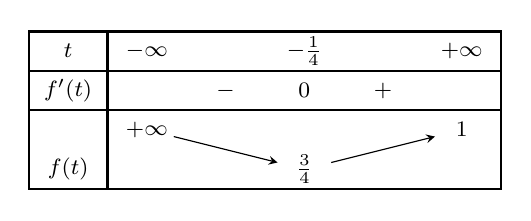
\begin{tikzpicture}[arrow/.style={>=stealth,->,shorten <= 10pt,shorten >= 10pt},font=\footnotesize,xscale=1,yscale=0.5]
		\foreach \i in {0,1,...,5}
		\foreach \j in {1,2,...,4} \coordinate (\i\j)at(\i,\j);
		\draw[thick] ([xshift=-0.5cm,yshift=-0.5cm]01)rectangle([xshift=0.5cm,yshift=0.5cm]54) ([xshift=0.5cm,yshift=-0.5cm]01)--([xshift=0.5cm,yshift=0.5cm]04) ([xshift=-0.5cm,yshift=-0.5cm]04)--([xshift=0.5cm,yshift=-0.5cm]54)([xshift=-0.5cm,yshift=-0.5cm]03)--([xshift=0.5cm,yshift=-0.5cm]53);
		\draw (04)node{$t$}(03)node{$f'(t)$}(01.5)node{$f(t)$};
		\foreach \nhan/\vtri in {$-\infty$/1,$-\frac{1}{4}$/3,$+\infty$/5}
		\draw (\vtri4)node{\nhan};
		\foreach \nhan/\vtri in {$-$/2,$0$/3,$+$/4}
		\draw (\vtri3)node{\nhan};
		\draw[arrow] (12)--(31);
		\draw[arrow] (31)--(52);
		\foreach \shf/\nhan/\vtri in {0cm/$+\infty$/12,0cm/$\frac{3}{4}$/31,0cm/$1$/52}
		\draw ([xshift=\shf]\vtri)node{\nhan};
	\end{tikzpicture}
	\end{center}
	Để phương trình có đúng 2 nghiệm $\dfrac{3}{4} < 2m < 1 \Leftrightarrow \dfrac{3}{8} < m< \dfrac{1}{2}$.
}
\end{ex}
\Closesolutionfile{ans}
\begin{indapan}{10}
	{ans/ans-1K1-3-Dang1}
\end{indapan}
